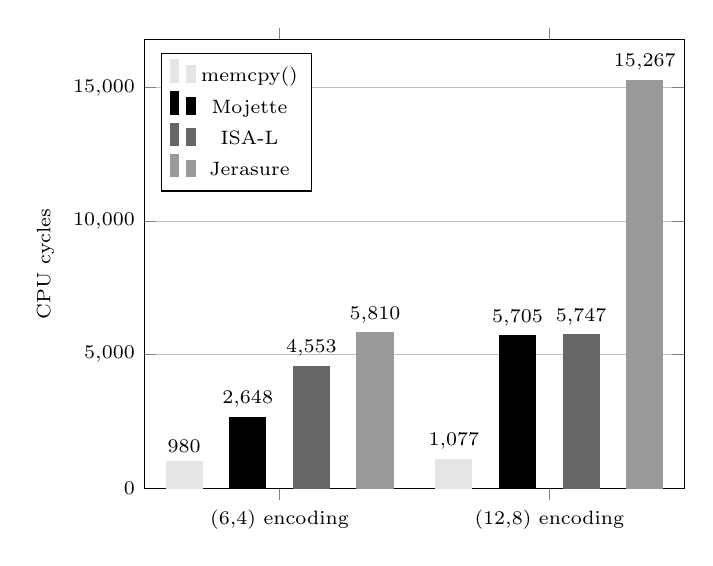
\begin{tikzpicture}
 \tikzstyle{every node}=[font=\scriptsize]
\begin{axis}[
    ybar=10pt,              % écarte les bars
    enlarge x limits=0.5,   % top ça ! écarte les côtés
    legend pos=north west,
    legend style={legend columns=1},
    ylabel={CPU cycles},
    symbolic x coords={1,2},
    bar width=13pt,
    ymin=0,
    %x tick label style={ rotate=45 },
    %y tick label style={ rotate=90 },
    xtick=data,%
    xticklabels={$(6{,}4)$ encoding,$(12{,}8)$ encoding},
    error bars/.cd,
    yminorgrids=true,
    ymajorgrids=true,
    nodes near coords,
    scaled y ticks=base 10:0,   % insane !
    cycle list = {black!10,black,black!60,black!40}
]

\addplot+[fill, text=black, error bars/.cd, y dir=both, y explicit]
 coordinates {
    (1,980)% +- (121,230)
    (2,1077)% +- (18,27)
};

\addplot+[fill, text=black, error bars/.cd, y dir=both, y explicit]
 coordinates {
    (1,2648)% +- (121,230)
    (2,5705)% +- (18,27)
};
\addplot+[fill, text=black, error bars/.cd, y dir=both, y explicit]
coordinates {
    (1,4553)% +- (20,32)
    (2,5747)%  +- (2,4)
};
\addplot+[fill, text=black, error bars/.cd, y dir=both, y explicit]
coordinates {
    (1,5810)% +- (14,16)
    (2,15267)%  +- (4,7)
};

\legend{memcpy(), Mojette, ISA-L, Jerasure}

\end{axis}
\end{tikzpicture}
